%!TEX root=paper/thesis.tex
\section{Method}\label{sec:clf_method}

We defer discussion of learning the \textbf{feature combination} classifier $g(\mathcal{H}_\pi) : 2^\mathcal{H} \mapsto \mathcal{Y}$ to~\autoref{sec:classifier}.
For now, we assume that $g$ can combine an arbitrary subset of features and provide a distribution $P(Y = y)$.
For example, $g$ could be a Naive Bayes (NB) model trained on the fully-observed data.

\todo{reference MDP formulation in \autoref{sec:mdp_formulation}.}

\todo{The set of \textbf{actions} $\mathcal{A}$ is exactly the set of features $\mathcal{H}$.}

%!TEX root=paper/thesis.tex
\subsection{Reward definition}\label{sec:clf_reward}

\begin{figure}[ht]
\centering
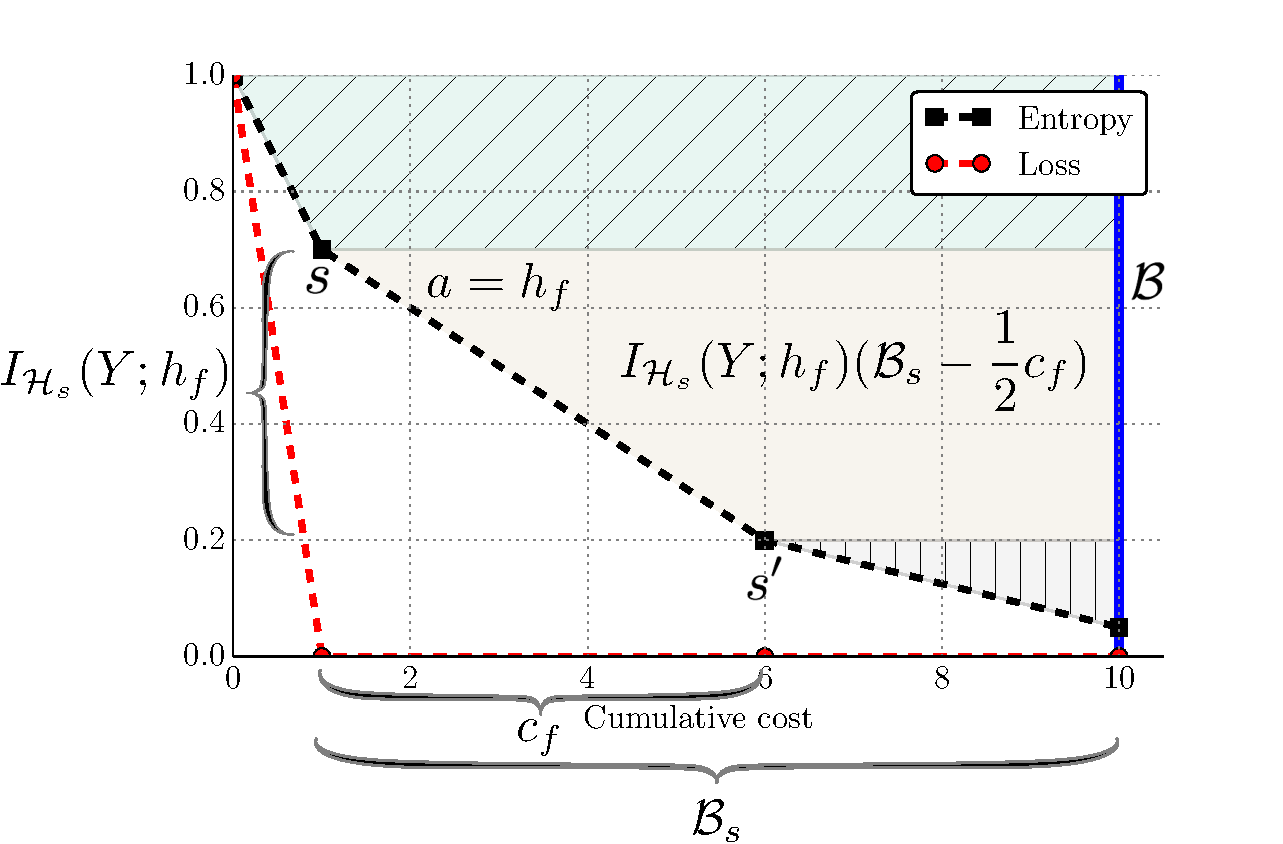
\includegraphics[width=.8\linewidth]{../../figures/rewards.pdf}
\caption{
Definition of the reward function.
To maximize the total area above the entropy vs. cost curve from $0$ to $\mathcal{B}$, we define the reward of an individual action as the area of the slice of the total area that it contributes.
From state $s$, action $a = h_f$ leads to state $s'$ with cost $c_f$.
The information gain is $I_{\mathcal{H}_s}(Y; h_f) = H(Y; \mathcal{H}_s) - H(Y; \mathcal{H}_s \cup {h_f})$.
\label{fig:clf_rewards}}
\end{figure}


\PM{Loss vs. cost}
The budget-sensitive loss $\mathcal{L}_\mathcal{B}$ enforces Anytime performance by valuing early gains more than later gains.
To formalize this, consider \hyperref[fig:clf_rewards]{Figure~\ref*{fig:clf_rewards}}, which shows the entropy and the 0-1 loss of $g$ at every point in a sequential feature selection episode for some instance $x$.
For the best Anytime performance, we want to capture the most area above the loss vs. cost curve, up to max budget $\mathcal{B}$ \parencite{Karayev-NIPS-2012}.
Recall from \eqref{eq:expected_reward} that the value of an episode $\xi$ is defined as the sum of obtained rewards.
If the reward of a single action is defined as the area above the curve that is captured as a direct result, then the value of the whole episode exactly corresponds to $\mathcal{L}_\mathcal{B}$.

\PM{Infogain}
However, there is a problem with using loss directly: only the first action to ``tip the scale'' toward the correct prediction gets a direct reward (in the figure, it is the first action).
A smoother reward function is desirable: if the classifier $g$ can give a full distribution $P(Y = y \mid \mathcal{H}_{\pi(x)})$ and not just a prediction $\hat{y} \in \mathcal{Y}$, we can maximize the \emph{information gain} of the selected subset instead of directly minimizing the loss of $g(\pi(x))$:
\begin{eqnarray}
I(Y; \mathcal{H}_{\pi(x)}) &=& H(Y) - H(Y | \mathcal{H}_{\pi(x)}) = \\ \notag
&=& \sum_{y \in Y} P(y) \log P(y) - \\ \notag
&&\sum_{y, \mathcal{H}_{\pi(x)}} P(y, \mathcal{H}_{\pi(x)}) \log P(y \mid \mathcal{H}_{\pi(x)})
\end{eqnarray}

\PM{Definition}
To the extent that $g$ is unbiased, maximizing information gain corresponds to minimizing loss, and ensures that we not only make the right classification decision but also become maximally certain.
Therefore, as graphically presented in \hyperref[fig:clf_rewards]{Figure~\ref*{fig:clf_rewards}}, we define the reward of selecting feature $h_s$ with cost $c_f$ with the set $\mathcal{H}_s$ computed to be $I_{\mathcal{H}_s}(Y; h_f) (\mathcal{B}_s - \frac{1}{2}c_f)$.
Although we do not evaluate in this regime, note that this definition easily incorporates a \textbf{setup cost} in addition to \textbf{deadline cost} by only computing the area in between setup and deadline costs.


%!TEX root=paper/paper.tex
\subsection{Features of the state}\label{sec:clf_features}

The featurization function $\phi(s)$ extracts the following features from the state:

\begin{itemize}\addtolength{\itemsep}{-.5\baselineskip}
\item Bit vector $\textbf{m}$ of length $F$: initially all bits are $1$ and are set to $0$ when the corresponding feature is computed.
\item For each $h_f$, a vector of size $d_f$ representing the values; $0$ until observed.
\item Cost feature $c \in [0, 1]$, for fraction of the budget spent.
\item Bias feature $1$.
\end{itemize}

\PM{Static vs Dynamic}
These features define the \textbf{dynamic} state, presenting enough information to have a \emph{closed-loop} (dynamic) policy that may select different features for different test instances.
The \textbf{static} state has all of the above features except for the observed feature values.
This enables only an \emph{open-loop} (static) policy, which is exactly the same for all instances.
Policy learned with the static state is used as a baseline in experiments.


\subsection{Learning the classifier.}\label{sec:classifier}

We have so far assumed that $g$ can combine an arbitrary subset of features and provide a distribution $P(Y = y)$---for example, a Gaussian Naive Bayes (NB) model trained on the fully-observed data.
However, a Naive Bayes classifier suffers from its restrictive independence assumptions.

Since discriminative classifiers commonly provide better performance, we use a \textbf{logistic regression} classifier, which presents a new challenge: at test time, some feature values are missing and need to be imputed.

If the classifier is trained exclusively on fully-observed data, then the feature value statistics at test time will not match, resulting in poor performance.
Therefore, we need to learn classifier weights on a distribution of data that exhibits the pattern of missing features induces by the policy $\pi$.
At the same time, learning the policy depends on the classifier $g$, used in the computation of the rewards.

\begin{algorithm}[]
\SetKwFunction{ComputeRewards}{ComputeRewards}
\SetKwFunction{GatherSamples}{GatherSamples}
\SetKwFunction{UpdatePolicy}{UpdatePolicy}
\SetKwFunction{UpdateClassifier}{UpdateClassifier}

\SetAlgoLined
\KwIn{$\mathcal{D} = \{x_n, y_n\}_{n=1}^N$; $\mathcal{L}_\mathcal{B}$}
\KwResult{Trained $\pi$, $g$}
\BlankLine
$\pi_0 \leftarrow$ random\;
\For {$i \leftarrow 1$ \KwTo max\_iterations} {
    States, Actions, Costs, Labels $\leftarrow$ \GatherSamples{$\mathcal{D}$, $\pi_{i-1}$}\;
    $g_i \leftarrow$ \UpdateClassifier{States, Labels}\;
    Rewards $\leftarrow$ \ComputeRewards{States, Costs, Labels, $g_i, \mathcal{L}_\mathcal{B}, \gamma$}\;
    $\pi_i \leftarrow$ \UpdatePolicy{States, Actions, Rewards}\;
}
\caption{Because reward computation depends on the classifier, and the distribution of states depends on the policy, $g$ and $\pi$ are trained iteratively.\label{alg:learning}}
\end{algorithm}


For this reason, the policy and classifier need to be learned jointly: \autoref{alg:learning} gives the iterative procedure.
In summary, we start from random $\pi$ and $g$, gather a batch of trajectories.
The batch is used to update both $g$ and $\pi$.
Then new trajectories are generated with the updated $\pi$, rewards are computed using the updated $g$, and the process is repeated.
This is a variant of generalized policy iteration \cite{Sutton1998}.

\paragraph{Unobserved value imputation.}
Unlike the Naive Bayes classifier, the logistic regression classifier is not able to use an arbitrary subset of features $\mathcal{H}_\pi$, but instead operates on feature vectors of a fixed size.
To represent the feature vector of a fully observed instance, we write $\mathbf{x} = [h_1(x), \dots, h_f(x)]$.
In case that $\mathcal{H}_\pi \subset \mathcal{H}$, we need to fill in unobserved feature values in the vector.

A basic strategy is \textbf{mean imputation}: filling in with the mean value of the feature:
\begin{align}
\mathbf{x}_\pi = \left[ h_i(x) : \left\{ \begin{array}{rl}
 h_i(x) &\mbox{ if $h_i \in \mathcal{H}_{\pi(x)}$} \\
 \bar{\mathbf{h}}_i &\mbox{ otherwise}
\end{array} \right. \right]
\end{align}

If we assume that $\mathbf{x}$ is distributed according to a multivariate Gaussian $\mathbf{x} \sim \mathcal{N}(\mathbf{0}, \Sigma)$, where $\Sigma$ is the sample covariance $X^T X$ and the data is standardized to have zero mean, then it is possible to do \textbf{Gaussian imputation}.
Given a feature subset $\mathcal{H}_\pi$, we write:
\begin{equation}
\mathbf{x}_\pi = \begin{bmatrix} \mathbf{x}^\text{o}\\  \mathbf{x}^\text{u} \end{bmatrix} \sim \mathcal{N} \left( \mathbf{0}, \begin{bmatrix} \mathbf{A} & \mathbf{C}\\ \mathbf{C}^T & \mathbf{B} \end{bmatrix} \right)
\end{equation}
where $\mathbf{x}^\text{o}$ and $\mathbf{x}^\text{u}$ represent the respectively observed and unobserved parts of the full feature vector $\mathbf{x}$.
%, $\mathbf{A}$ is the covariance matrix of $\mathbf{x}^\text{o}$, $\mathbf{B}$ is the covariance matrix of $\mathbf{x}^\text{u}$, and $C$ is the cross-variance matrix that has as many rows as the size of $\mathbf{x}^\text{o}$ and as many columns as the size of $\mathbf{x}^\text{u}$.
%\parencite{Roweis-gaussian-identities}.
In this case, the distribution over unobserved variables conditioned on the observed variables is given as
$\mathbf{x}^\text{u} \mid \mathbf{x}^\text{o} \sim \mathcal{N} \left( \mathbf{C}^T \mathbf{A}^{-1} \mathbf{x}^\text{o},\, \mathbf{B} - \mathbf{C}^T \mathbf{A}^{-1} \mathbf{C} \right)$.

\paragraph{Learning more than one classifier.}
As illustrated in \hyperref[fig:state_space]{Figure~\ref*{fig:state_space}}, the policy $\pi$ selects some feature subsets more frequently than others.
Instead of learning only one classifier $g$ that must be robust to all observed feature subsets, we can learn several classifiers, one for each of the most frequent subsets.
This is done by maintaining a distribution over encountered feature subsets during training.
For each of the $K$ most frequent subsets, a separate classifier is trained, using data that is closest by Hamming distance on the selected-feature bit vector.

Each classifier is trained with the \textsc{Liblinear} implementation of logistic regression, with $L_2$ regularization parameter K-fold cross-validated at each iteration.

\begin{figure}[ht]
\centering
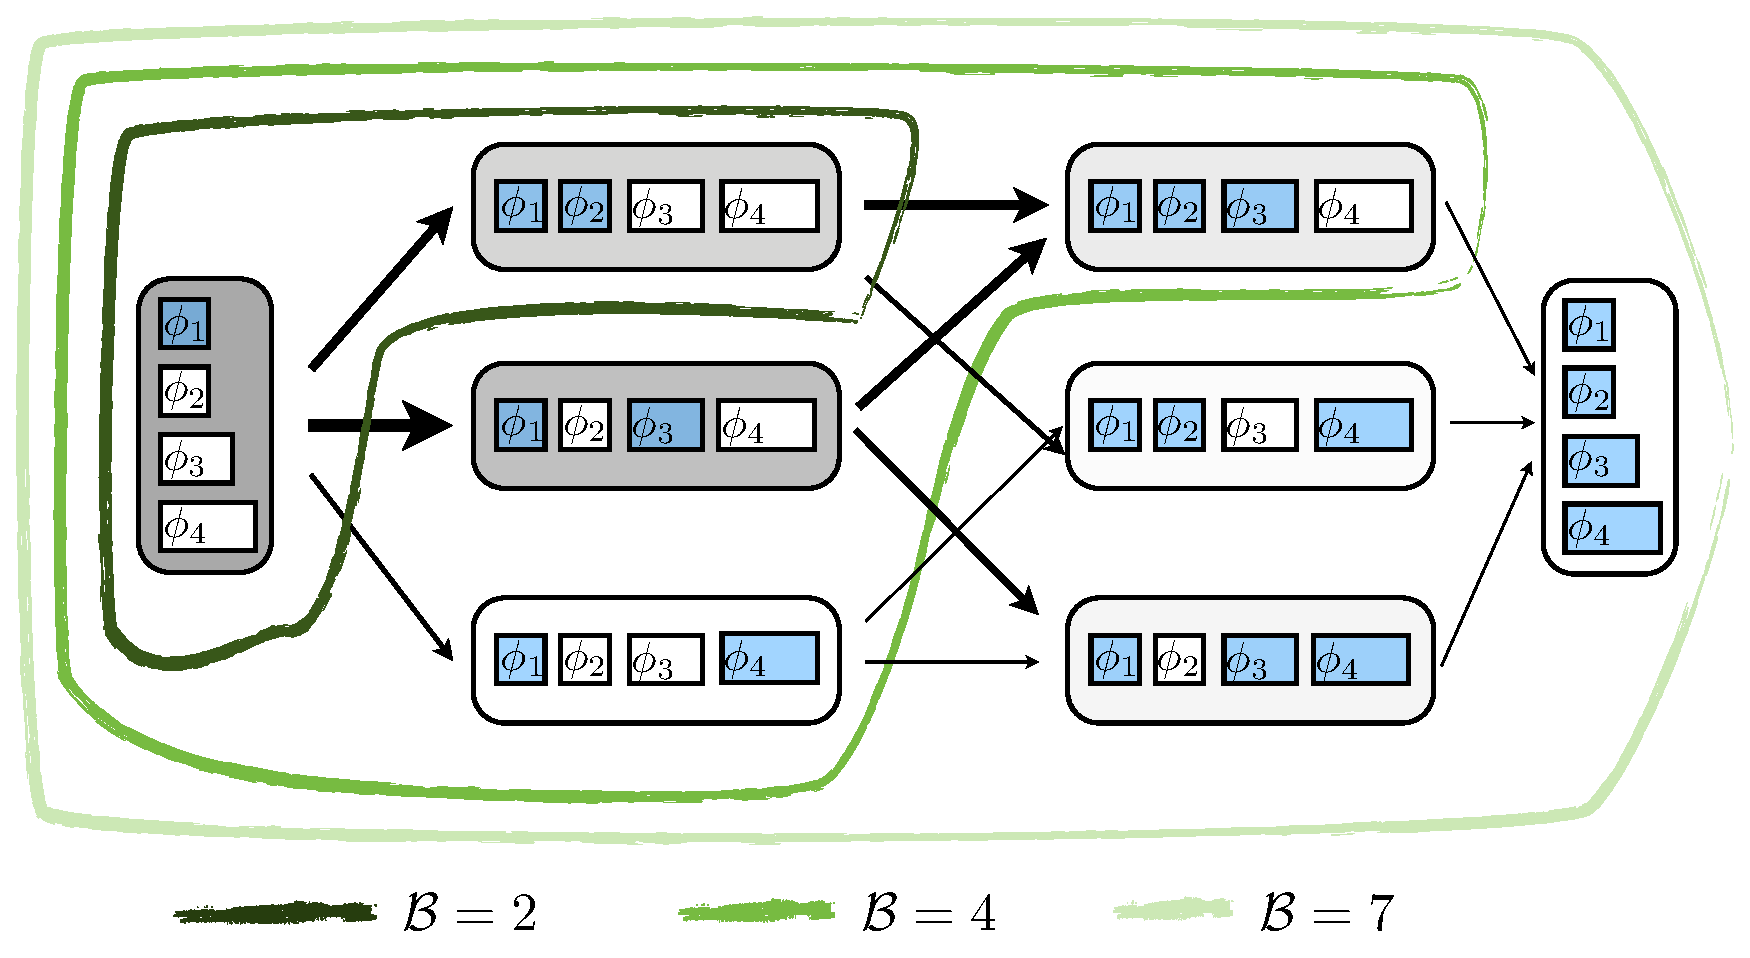
\includegraphics[width=1\linewidth]{../../figures/mdp_masks.pdf}
\caption{
The action space $\mathcal{A}$ of the MDP is the the set of features $\mathcal{H}$, represented by the $\phi$ boxes.
The primary discretization of the state space can be visualized by the possible feature subsets (larger boxes); selected features are colored in the diagram.
The feature selection policy $\pi$ induces a distribution over feature subsets, for a dataset, which is represented by the shading of the larger boxes.
Not all states are reachable for a given budget $\mathcal{B}$.
In the figure, we show three ``budget cuts'' of the state space.
\label{fig:state_space}
}
\end{figure}


% %!TEX root=paper/paper.tex
\chapter{Prediction with Features Missing at Test Time}

\section{Abstract}
We look at prediction with all features available at training time, but only a subset observed at test time.
Such situations may arise due to sensor loss, or when using test-time instance-specific feature selection.
We examine three areas of modeling choices:

\begin{enumerate}
\item For imputation, we look at mean, SVD, joint Gaussian conditioning, and nearest neighbor methods.

\item For classification, we evaluate augmenting the training data with imputed values, modifying the loss function to consider the expected feature ``corruption'', and using non-linear classifiers.

\item We additionally evaluate training different classifiers for different subsets of observed features.
\end{enumerate}

We evaluate reconstruction and classification error on two datasets: Digits and Scenes-15.
Two feature selection policies are considered: Random and Clustered.
For each policy, we consider Independent and Block-wise selection patterns.

We find that mean imputation with classifier retraining is a reasonably well-performing approach.
Nearest Neighbor methods perform best but are the most expensive.
Gaussian imputation method performs very well, but is also expensive.

Training classifiers with a loss function modified to expect a certain level of feature corruption did not improve performance.
Training additional classifiers for clusters of observed feature subsets did not improve performance.

\section{Introduction}
In supervised prediction problems, \emph{features} extracted from inputs are combined to output a real value (regression) or a label (classification).
The goal of training is to minimize the \emph{loss} of the predictions with the true values or labels---for example, the accuracy of classification.

We look at a complication of this problem.
While all features are available at training time, only a subset of features of each instance is observed at test time.
Such situations can arise in real world deployments of predictive systems due to sensor failure.
Another motivation for the problem comes from work on dynamic feature selection: to predict with minimum loss on a fixed time budget, different subsets of features are extracted for different instances \parencite{Karayev-NIPS-2012, Xu-ICML-2013}.

Since the training set is fully observed, we can train a classifier with all features.
At test time, we could attempt to impute the unobserved feature values given the observed ones, and use the classifier trained on the fully observed training set.
There are many methods of imputing missing values, differing in their power and cost.
We consider: simple mean imputation; singular value decomposition-based imputation; multivariate Gaussian conditioning; and nearest neighbor imputation with two similarity measures.

In addition to imputing at test time, we can apply the test-time observation process to the training data, impute values, and re-train the classifier.
This amounts to a regularization that prevents the classifier from relying on any single feature, as it may not be in the observed subset.
Taking this idea further, we could work the expected feature ``corruption'' into the loss function of the linear classifier, which is equivalent to augmenting the training set with an infinite amount of corrupted data.

The feature selection process may not select features independently.
It could select features by block instead of one by one, and it could have a bound on the total number of unique subsets that are selected.
We evaluate in these conditions, and notice that if there is a small bound on the number of subsets, then we can learn a separate classifier for each subset of observed features.
Even if the bound is not small, we may still derive benefit from training more than one classifier, and at test time using the classifier trained on the closest subset of features to the observed instance.

\section{Problem Formulation}

\begin{mydef} \label{def:problem}
\textbf{The prediction problem} consists of
\begin{itemize}
\item Set $\mathcal{D}$ of $N$ instances of $K$ possible labels: $\mathcal{D} = \{x_n \in \mathcal{X}, y_n \in \{1, \dots, K\}\}_{n=1}^N$.

\item Set $\mathcal{H}$ of $F$ features $\mathcal{H} = \{h_f : \mathcal{X} \mapsto \mathbb{R} \}_{f=1}^F$.\\
To represent featurized instance, we write $\mathbf{x} = [h_0(x), h_1(x), \dots, h_f(x)]$.

\item Test-time feature selection function $o(x, b): \mathcal{X} \times \mathbb{R} \mapsto \mathbb{B}^F$, where $\mathbb{B} \in \{0, 1\}$, and $b \in [0, 1]$ is given and specifies the fractional selection \emph{budget}.

\item Loss function $\ell(g(x), y): \mathbb{R}^K \times \{1, \dots, K\} \mapsto \mathbb{R}$.
\end{itemize}

Given $b$, we seek a procedure $g(x)$ that minimizes total loss $\sum \ell(g(x_n), y_n)$ under the condition that $o(x, b)$ is applied to each $x$.
\end{mydef}

Applied to $x$, $o(x, b)$ gives the binary selection vector $\mathbf{o}$ which splits $\mathbf{x}$ it into observed and unobserved parts such that $\mathbf{x}^m = [\mathbf{x}^\text{o}, \mathbf{x}^\text{u}]$.

$X^c$ denotes the fully observed $N \times F$ training set.
We assume that we have only sequential access to the missing-feature test instances $\mathbf{x}^m$.

We see three experimental conditions: (1) how to fill in missing values; (2) which loss function to use in learning the classifier and whether to augment the training data; (3) how many classifiers to learn.


\section{Classifiers}

In addition to the $k$-NN classifier described above, we consider three linear classifiers, obtained by minimizing:
\begin{enumerate}
  \item Logistic loss on fully observed data: simply using $X^c$.
  \item Logistic loss on synthetically re-imputed version of the data: we obtain $X^m$ through applying $o(x, b)$ on each $x^c$, and then imputing the missing values with the methods described.
  \item Logistic and quadratic loss derived with Marginalized Corrupted Features (MCF) \parencite{Maaten-ICML-2013}.
\end{enumerate}

The idea of (3) is to move the expectation of feature corruption into the loss function, which is equivalent to adding an infinite amount of corrupted data to the training set.
Remarkably, this is not any more computationally complex than the standard loss (although minimization does take longer, empirically).

For example, for blankout noise and logistic loss, we can derive the surrogate loss
\begin{equation}
\mathcal{L}(D; \mathbf{\theta}) \leq \sum_{n=1}^N \log \left( 1 + \prod_{f=1}^F \left[ q_f + (1 - q_f) e^{-y_n \theta_f \frac{1}{1 - q_d} x_{nf}} \right] \right)
\end{equation}

For additional loss functions, see \parencite{Maaten-ICML-2013}.

\subsection{Clustering classifiers}

\section{Evaluation}





